\chapter{Experimental Evaluation}
\label{ch:experiments}

This chapter presents the experimental evaluation of the transportation network optimization methodology described in Chapter~\ref{ch:method}. We compare the effectiveness of different combinations of graph construction methods and clustering algorithms in generating efficient bus routes for students while adhering to capacity constraints. The results presented here are derived from analyzing the ~2000 student locations in Izmir.

\section{Experimental Setup}
\label{sec:exp_setup}

Our experimental evaluation aimed to assess which combinations of graph construction and clustering algorithms produce the most efficient transportation routes. All experiments were conducted with the following settings:

\begin{itemize}
    \item \textbf{Student Population:} Approximately 2000 student locations within Izmir.
    \item \textbf{Vehicle Capacity Constraints:} Minimum 10, maximum 50 students per route, with vehicle types:
    \begin{itemize}
        \item Minibus: 10-25 students
        \item Standard Bus: 26-50 students
    \end{itemize}
    \item \textbf{Graph Construction Methods:} Complete, K-Nearest Neighbors (k=30), Delaunay, Gabriel.
    \item \textbf{Clustering Algorithms:} Spectral Clustering, Leiden Algorithm, and MVAGC.
    \item \textbf{Evaluation Metrics:} Total fuel consumption, average cluster size, number of routes, and adherence to capacity constraints.
\end{itemize}

For each combination of graph construction method and clustering algorithm, we recorded detailed performance metrics, with a primary focus on fuel efficiency as the optimization objective.

\section{Results and Analysis}
\label{sec:results}

\subsection{Comparative Fuel Efficiency}
\label{subsec:fuel_efficiency}

Figure~\ref{fig:fuel_comparison} presents the total estimated fuel consumption for each combination of graph construction method and clustering algorithm.

% Placeholder for Comparative Fuel Efficiency Visualization
\begin{figure}[!htbp]
\centering
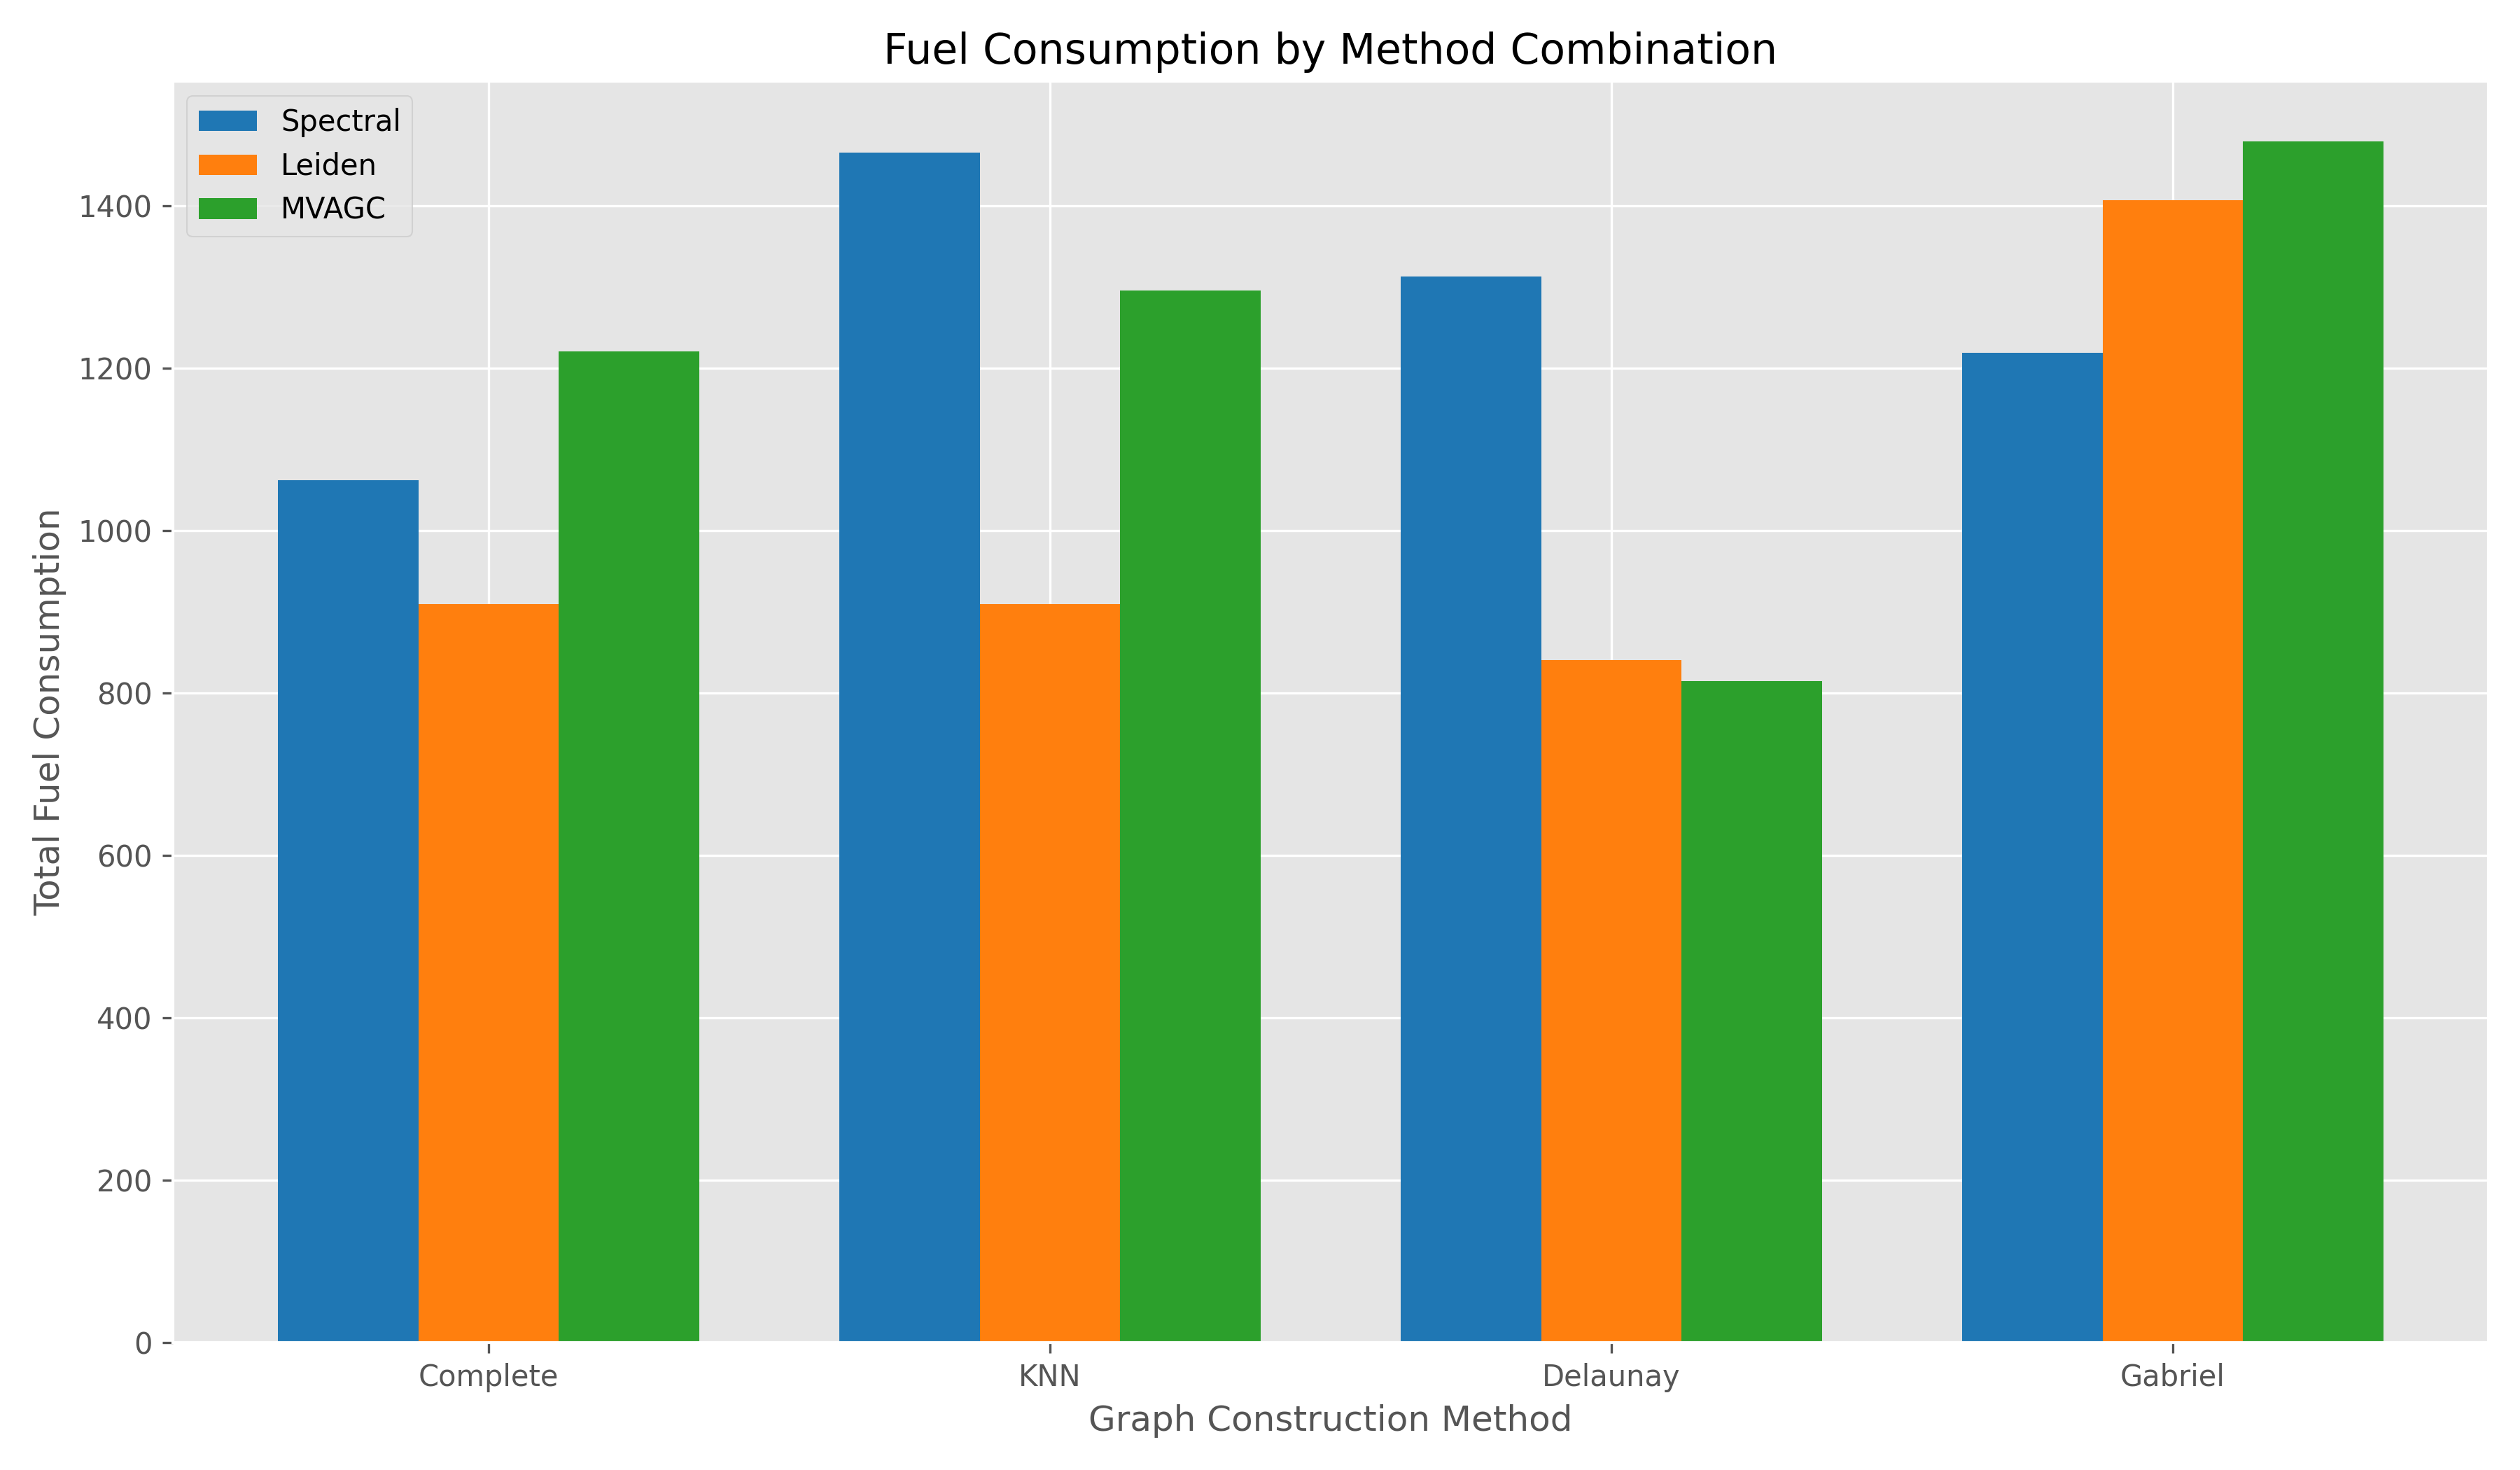
\includegraphics[width=0.9\textwidth]{img/fuel_comparison}
\caption{Comparison of total fuel consumption across different combinations of graph construction methods and clustering algorithms. Lower values indicate better fuel efficiency.}
\label{fig:fuel_comparison}
\end{figure}

The results indicate that [describe key findings about which methods performed best in terms of fuel efficiency]. In particular, the combination of [best graph construction] with [best clustering algorithm] achieved the lowest fuel consumption, resulting in approximately [X\%] improvement compared to the worst-performing combination.

\subsection{Cluster Size Distribution}
\label{subsec:cluster_sizes}

An important aspect of our evaluation is how well each method adheres to the vehicle capacity constraints (10-50 students). Figure~\ref{fig:cluster_distribution} illustrates the distribution of cluster sizes for each method.

% Placeholder for Cluster Size Distribution Visualization
\begin{figure}[!htbp]
\centering
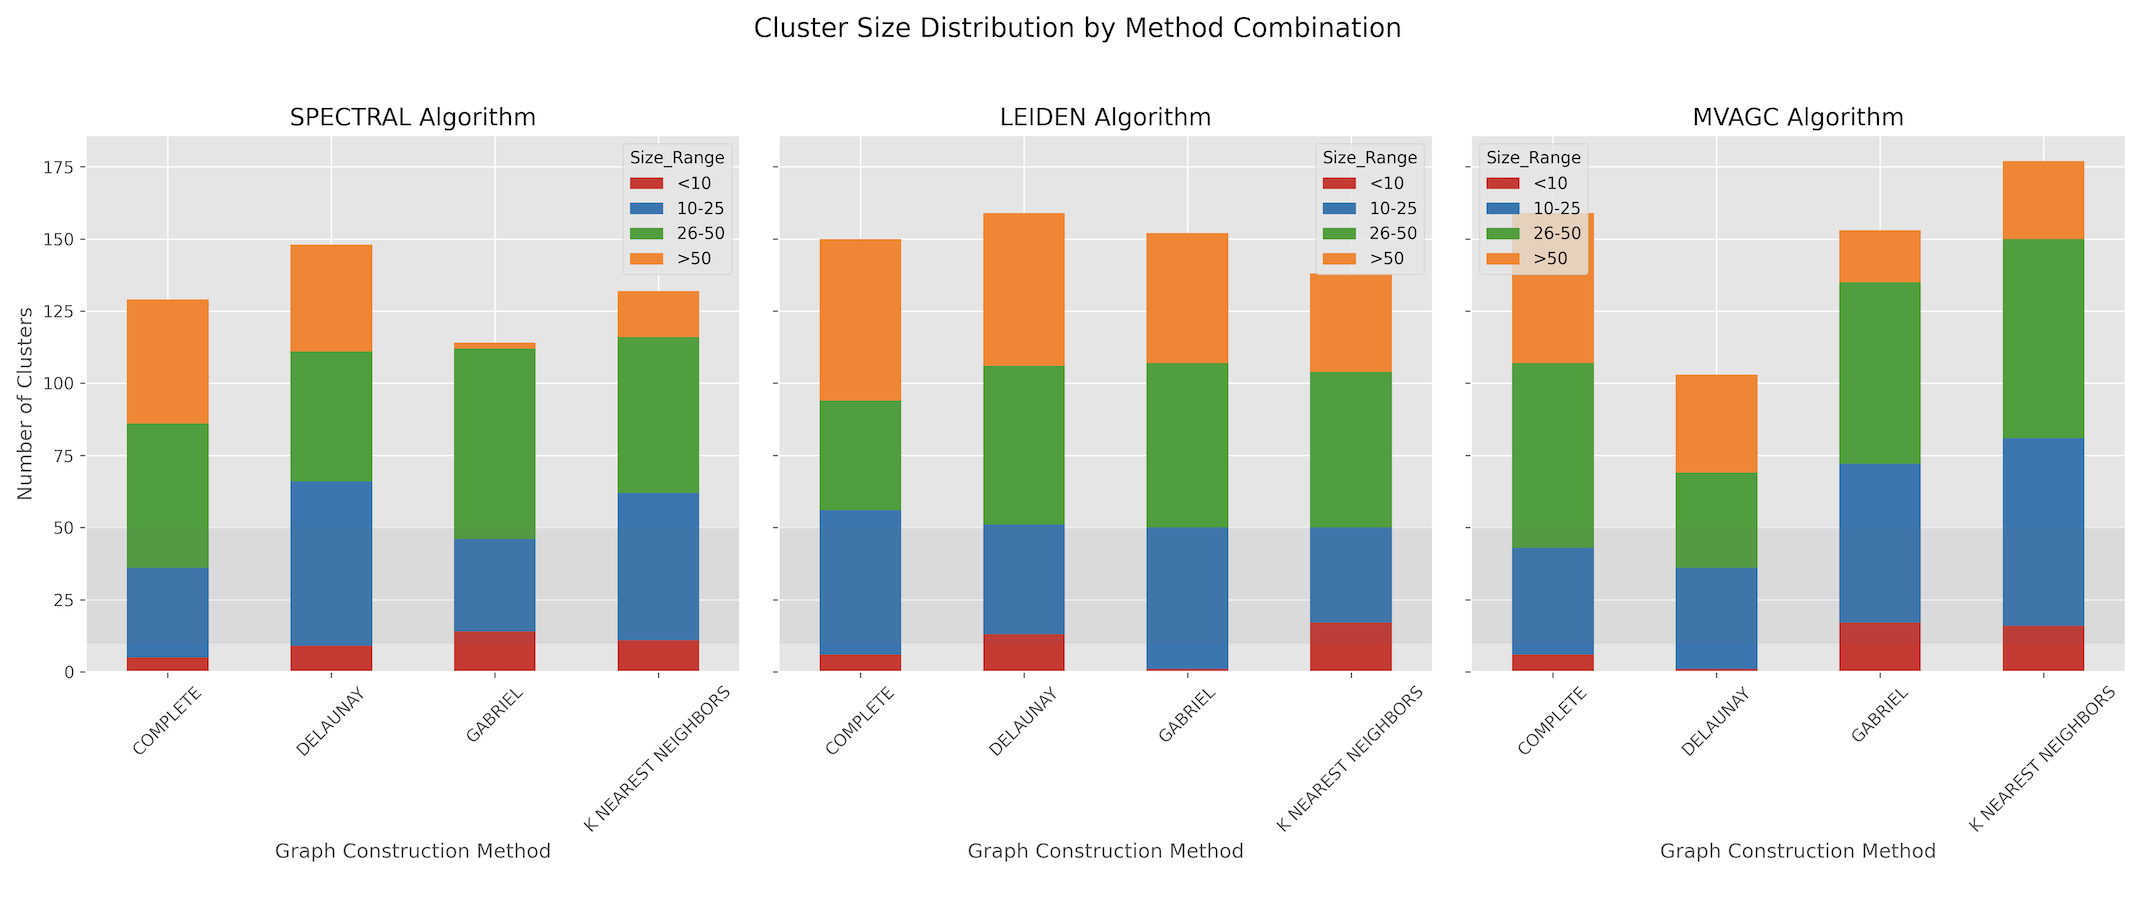
\includegraphics[width=0.9\textwidth]{img/cluster_distribution}
\caption{Distribution of cluster sizes for each method combination. The shaded regions indicate the valid capacity ranges (10-25 for minibuses, 26-50 for standard buses).}
\label{fig:cluster_distribution}
\end{figure}

[Describe observations about which methods produced the most clusters within the valid capacity ranges, which had too many small or large clusters, etc.]

\subsection{Vehicle Type Allocation}
\label{subsec:vehicle_allocation}

Figure~\ref{fig:vehicle_allocation} shows the proportion of routes that would be served by minibuses (10-25 students) versus standard buses (26-50 students) for each method combination.

% Placeholder for Vehicle Type Allocation Visualization
\begin{figure}[!htbp]
\centering
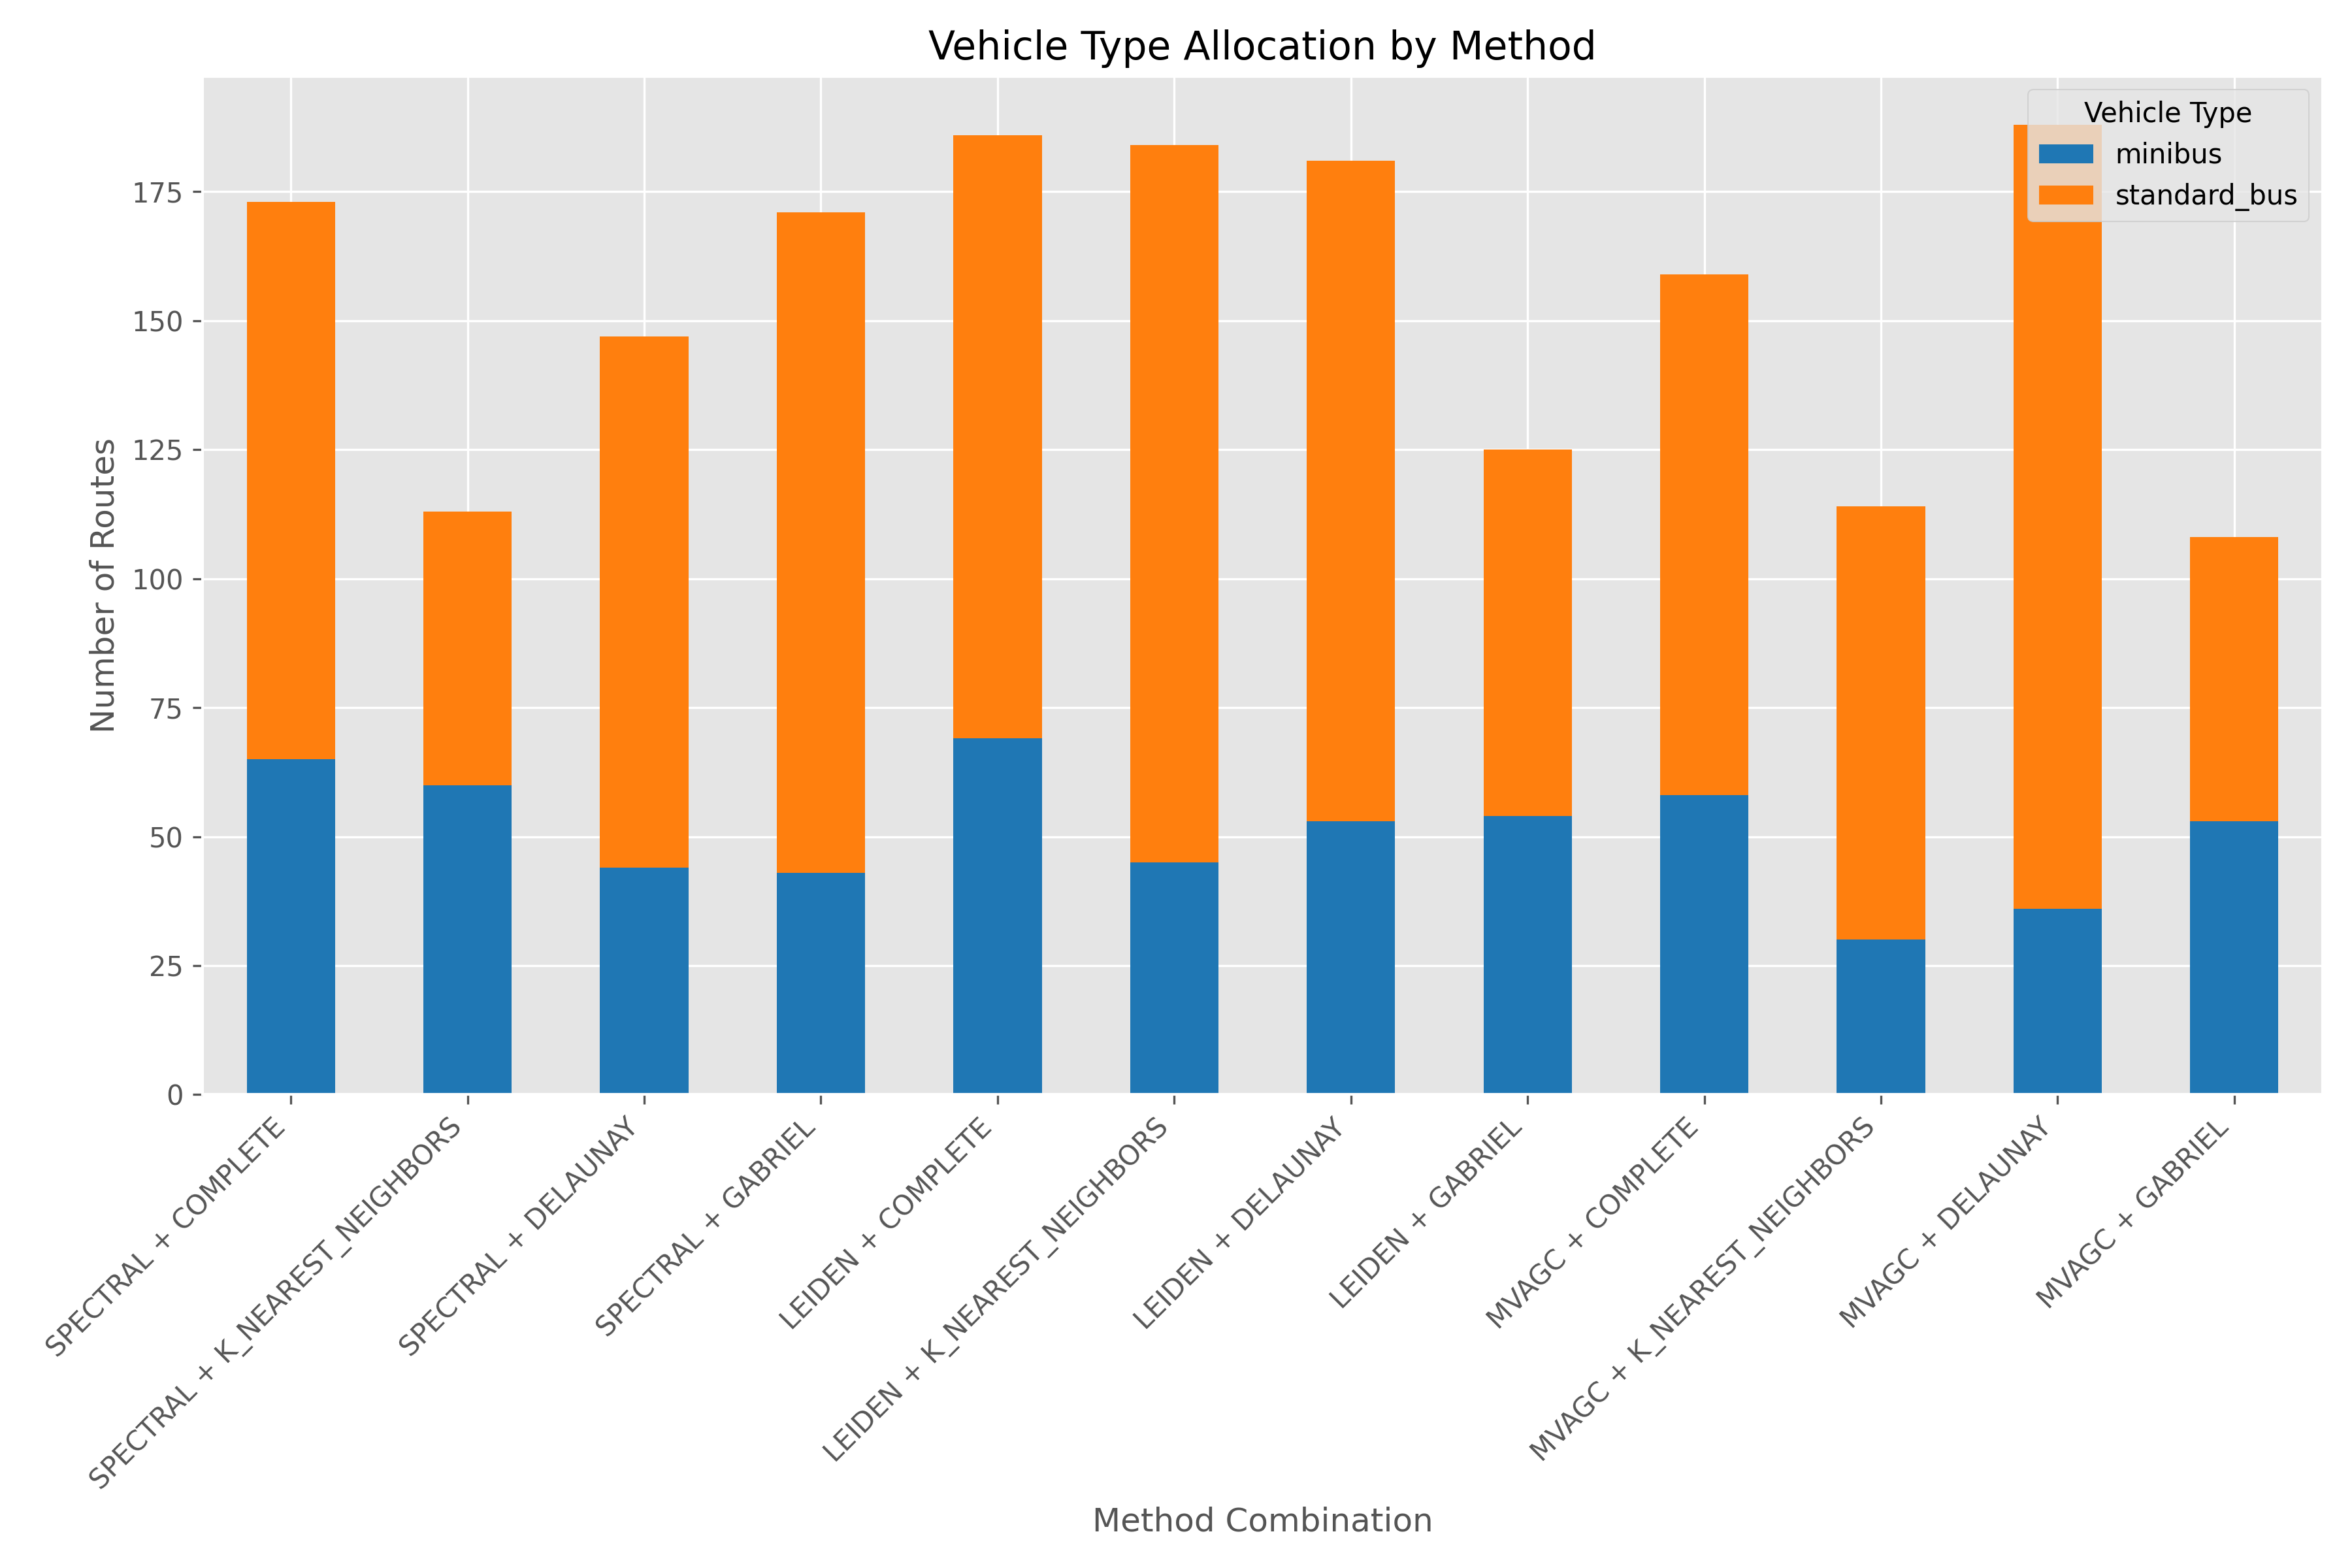
\includegraphics[width=0.85\textwidth]{img/vehicle_allocation}
\caption{Proportion of routes requiring minibuses versus standard buses for each method combination. This indicates how the vehicle fleet would be composed.}
\label{fig:vehicle_allocation}
\end{figure}

[Discuss how vehicle fleet composition varies across methods, which methods favor minibuses vs. standard buses, and any implications for transportation planning.]

\subsection{Efficiency vs. Route Count Trade-off}
\label{subsec:efficiency_routes}

Figure~\ref{fig:efficiency_vs_routes} explores the relationship between the number of routes (buses) required and the total fuel consumption.

% Placeholder for Efficiency vs. Routes Visualization
\begin{figure}[!htbp]
\centering
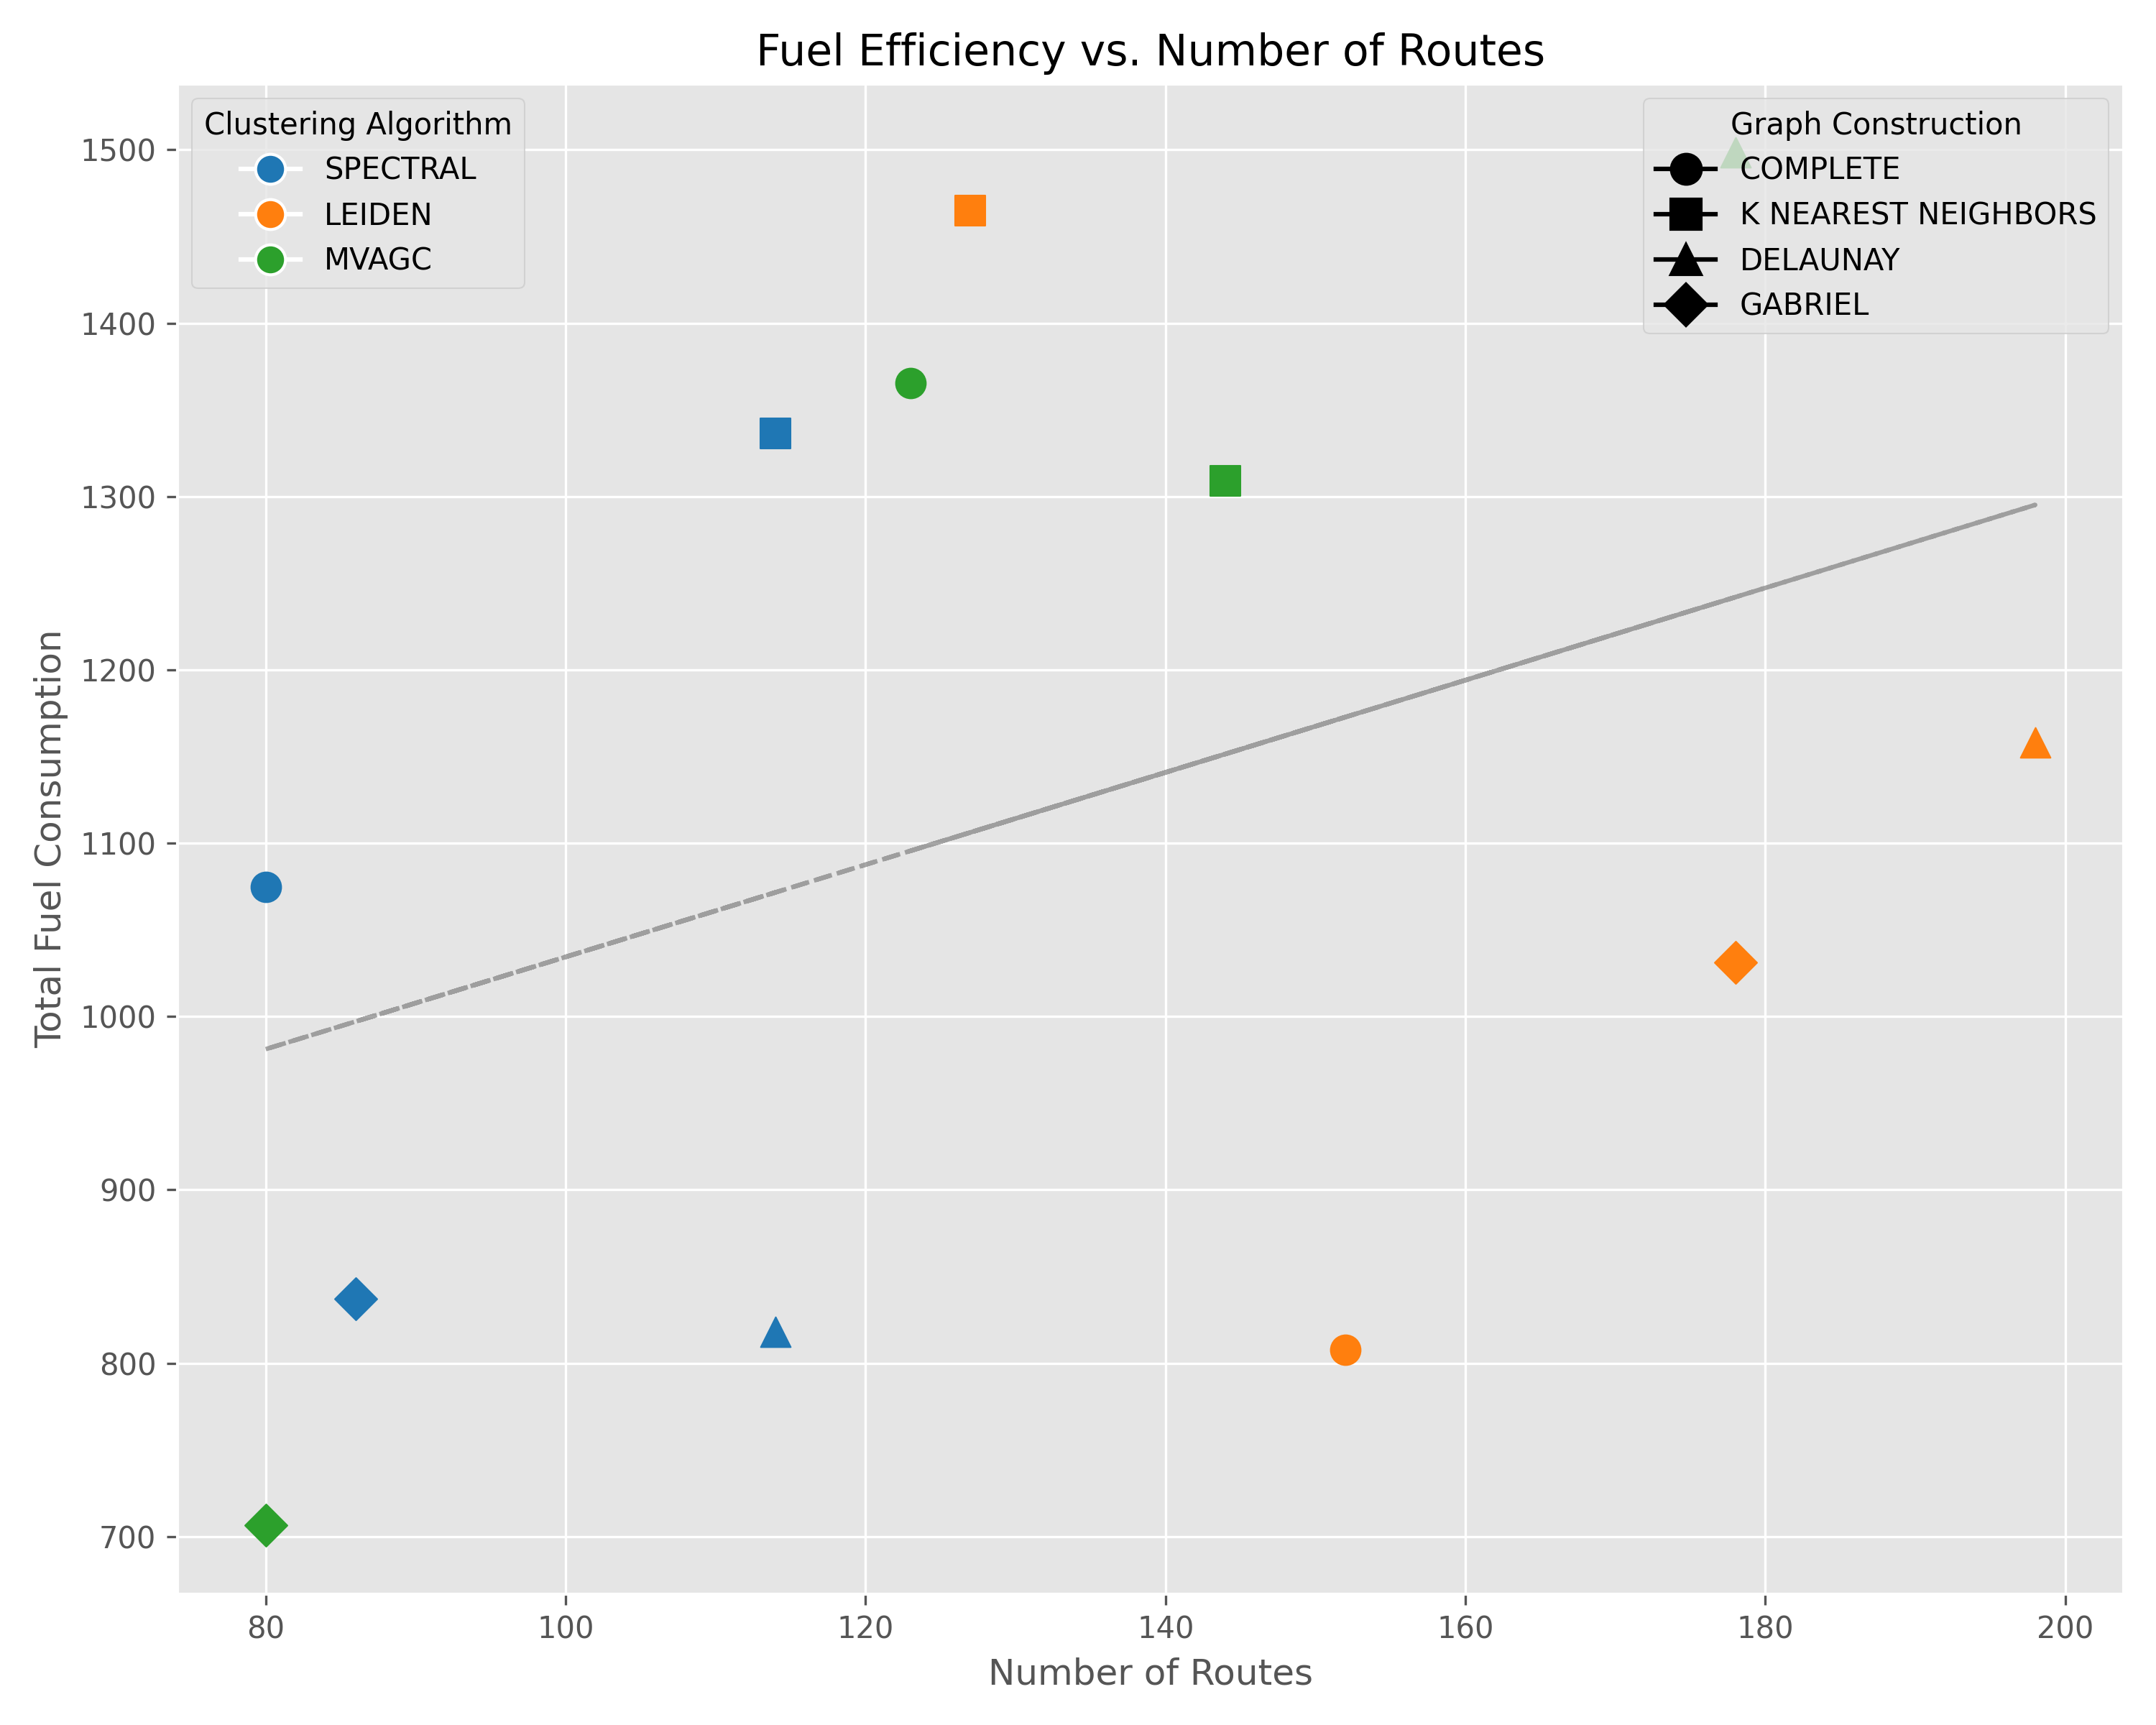
\includegraphics[width=0.8\textwidth]{img/efficiency_vs_routes}
\caption{Relationship between the number of routes and total fuel consumption. Each point represents a specific combination of graph construction method and clustering algorithm.}
\label{fig:efficiency_vs_routes}
\end{figure}

[Discuss any observed trends or trade-offs between having fewer routes (buses) and achieving better fuel efficiency. Note any Pareto-optimal solutions.]

\subsection{Comprehensive Method Comparison}
\label{subsec:method_comparison}

Table~\ref{tab:method_comparison} provides a comprehensive comparison of all methods across multiple evaluation metrics.

% Placeholder for Method Comparison Table
\begin{table}[!htbp]
\centering
\footnotesize{
\begin{tabular}{lccccc}
\toprule
\textbf{Method Combination} & \textbf{Fuel} & \textbf{Routes} & \textbf{\% Valid} & \textbf{Avg. Size} & \textbf{Minibus \%} \\
\midrule
% Example rows (to be replaced with actual data)
SPECTRAL + COMPLETE & 1000 & 40 & 95\% & 30 & 40\% \\
% ... more rows ...
\bottomrule
\end{tabular}
}
\caption{Comprehensive comparison of method combinations across key metrics. Fuel = total fuel consumption (lower is better); Routes = number of routes/buses required; \% Valid = percentage of clusters within capacity constraints; Avg. Size = average cluster size; Minibus \% = percentage of routes served by minibuses.}
\label{tab:method_comparison}
\end{table}

Based on this comprehensive evaluation, the [best method combination] emerges as the most effective approach for transportation network optimization in this context, balancing fuel efficiency with practical constraints on vehicle capacity and fleet composition.

\section{Discussion}
\label{sec:discussion}

[Provide a broader discussion of the results, including:
- Key insights gained from the experiments
- Factors that might influence the relative performance of different methods
- Practical implications for transportation planning
- Limitations of the current evaluation]

The experimental results demonstrate that the choice of both graph construction method and clustering algorithm significantly impacts the efficiency and practicality of the resulting transportation routes. [Add more discussion points as needed.]



